\section{Trigonometrie und Hyperbelfunktionen}
	\begin{minipage}[t]{0.55\textwidth}
		\textbf{Kosinussatz}:\quad $c^{2}=a^{2}+b^{2}-2ab\cos(\gamma)$\\
		\textbf{Sinussatz}:\qquad $\frac{a}{\sin(\alpha)}=\frac{b}{\sin(\beta)}=\frac{c}{\sin(\gamma)}$\\[8pt]
		\textbf{Rechtwinkliges Dreieck}:
		\begin{tabbing}
			xxxxxxxxxxxxxxxxxxxxxxxxxx \= \kill
			$\sin(\beta)=\frac{b}{a}=\frac{Gegenkathete}{Hypotenuse}$\> $\tan(\beta)=\frac{b}{c}=\frac{Gegenkathete}{Ankathete}$\\
			$\cos(\beta)=\frac{c}{a}=\frac{Ankathete}{Hypotenuse}$\>
			$\cot(\beta)=\frac{c}{b}=\frac{Ankathete}{Gegenkathete}$\\
			\\
			$\sin^{2}(x)+\cos^{2}(x)=1$ \> $\tan(x)=\frac{\sin(x)}{\cos(x)}$
		\end{tabbing}
	\end{minipage}
%
	\begin{minipage}[t]{0.45\textwidth}
		\begin{flushright}
			\strut\vspace*{-\baselineskip}\newline
			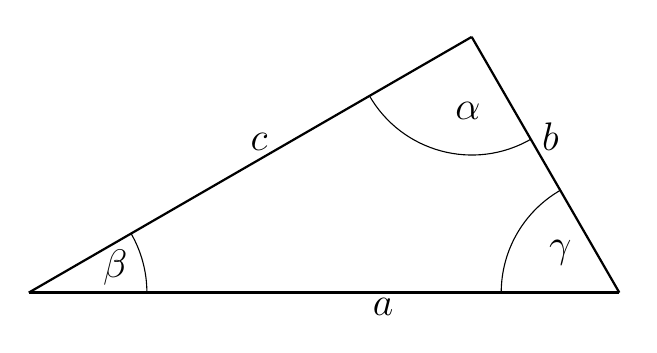
\begin{tikzpicture}[xscale=0.75, yscale=0.75]
	%axis
	\draw[thick, -] (0, 0) -- (10,0) node[label={[xshift=-3cm, yshift=-0.55cm]\Large $a$}]{};
	\draw[thick, -] (10, 0) -- (7.5,4.33) node[label={[xshift=1cm, yshift=-1.7cm]\Large $b$}]{};
	\draw[thick, -] (0, 0) -- (7.5,4.33) node[label={[xshift=-2.7cm, yshift=-1.7cm]\Large $c$}]{};
	
	\draw (2,0) arc (0:30:2cm) node[label={[xshift=-0.2cm, yshift=-0.9cm]\Large $\beta$}]{};
	\draw (8,0) arc (180:120:2cm) node[label={[xshift=0cm, yshift=-1.2cm]\Large $\gamma$}]{};
	\draw (5.77,3.33) arc (210:300:2cm) node[label={[xshift=-0.8cm, yshift=0cm]\Large $\alpha$}]{};;
	%
	
	%
	%plots
	%\draw[red, domain=-4:1.4] plot (\x, {e^\x}) node[right, red] {\Large $e^x$};
	%\draw[blue, domain=0.03:4] plot (\x, {ln(\x)})node[above, blue] {\Large $ln(x)$};
\end{tikzpicture}
		\end{flushright}
	\end{minipage}
%
\subsection{Quadrantenbeziehungen}
\begin{tabbing}
	xxxxxxxxxxxxxxxxxxxxxxxxxxxxxxxxxx \= \kill
	$\sin(-a)=-\sin(a)$ \> $\cos(-a)=\cos(a)$\\
	$\sin(\pi - a)=\sin(a)$ \> $\cos(\pi - a)=-\cos(a)$\\
	$\sin(\pi + a)=-\sin(a)$ \> $\cos(\pi +a)=-\cos(a)$\\
	$\sin\left(\frac{\pi}{2}-a \right)=\sin\left(\frac{\pi}{2}+a \right)=\cos(a)$ \>
	$\cos\left(\frac{\pi}{2}-a \right)=-\cos\left(\frac{\pi}{2}+a \right)=\sin(a)$\\
	$\sinh(a)=-\sinh(-a)$ \> $\cosh(-a)=\cosh(a)$
\end{tabbing}

\begin{minipage}[t]{0.5\textwidth}
\subsection{Additionstheoreme}
	$\sin(a \pm b)=\sin(a) \cdot \cos(b) \pm \cos(a) \cdot \sin(b)$\\
	$\cos(a \pm b)=\cos(a) \cdot \cos(b) \mp \sin(a) \cdot \sin(b)$\\	
	$\tan(a \pm b)=\dfrac{\tan(a) \pm \tan(b)}{1 \mp \tan(a) \cdot \tan(b)}$\\
	$\sinh(a \pm b)=\sinh(a) \cdot \cosh(b) \pm \cosh(a) \cdot \sinh(b)$\\
	$\cosh(a \pm b)=\cosh(a) \cdot \cosh(b) \mp \sinh(a) \cdot \sinh(b)$\\	
	$\tanh(a \pm b)=\dfrac{\tanh(a) \pm \tanh(b)}{1 \pm \tanh(a) \cdot \tanh(b)}$\\
\end{minipage}
%
\begin{minipage}[t]{0.5\textwidth}
	\subsection{Euler-Formeln} 
	$\sin(x) = \frac{1}{2j} \left(e^{jx} - e^{-jx}\right)$ \\
	$\cos(x) = \frac{1}{2} \left(e^{jx} + e^{-jx}\right)$ \\
	$\sinh(x) = \frac{1}{2} \left(e^{x} - e^{-x}\right)$ \\
	$\cosh(x) = \frac{1}{2} \left(e^{x} + e^{-x}\right)$ \\
	$e^{x+jy} = e^x \cdot e^{jy} = e^x \cdot \left(\cos(y) + j\sin(y)\right)$ \\
	$e^{j\pi} = e^{-j\pi} = -1$ \\
\end{minipage}
\\[10pt]
%
\begin{minipage}[t]{0.5\textwidth}
\subsection{Periodizität}
	\begin{tabbing}
		xxxxxxxxxxxxxxxxxxxxxxxx \= \kill
		$\cos(a+k\cdot2\pi)=\cos(a)$ \> $(k \in \mathbb{Z})$\\
		$\sin(a+k\cdot2\pi)=\sin(a)$ \> $(k \in \mathbb{Z})$
	\end{tabbing}	
\end{minipage}
%
\begin{minipage}[t]{0.5\textwidth}
	\subsection{Doppel- und Halbwinkel}	
	$\sin(2a)=2\sin(a)\cos(a)$\\
	$\cos(2a)=\cos^2(a)-\sin^2(a)=2\cos^2(a)-1=1-2\sin^2(a)$\\
	$\cos^2 \left(\frac{a}{2}\right)=\frac{1+\cos(a)}{2} \qquad
	\sin^2 \left(\dfrac{a}{2}\right)=\frac{1-\cos(a)}{2}$
\end{minipage}
\\[10pt]
%
\begin{minipage}[t]{0.5\textwidth}
\subsection{Summe und Differenz}
	$\sin(a)+\sin(b)=2 \cdot \sin \left(\frac{a+b}{2}\right) \cdot
	\cos\left(\frac{a-b}{2}\right)$\\
	$\sin(a)-\sin(b)=2 \cdot \sin \left(\frac{a-b}{2}\right) \cdot \cos\left(\frac{a+b}{2}\right)$\\
	$\cos(a)+\cos(b)=2 \cdot \cos \left(\frac{a+b}{2}\right) \cdot
	\cos\left(\frac{a-b}{2}\right)$\\
	$\cos(a)-\cos(b)=-2 \cdot \sin \left(\frac{a+b}{2}\right) \cdot
	\sin\left(\frac{a-b}{2}\right)$\\
	$\tan(a) \pm \tan(b)=\dfrac{\sin(a \pm b)}{\cos(a)\cos(b)}$
\end{minipage}
%
\begin{minipage}[t]{0.5\textwidth}
\subsection{Produkte}
$\sin(a)\sin(b)=\frac{1}{2}(\cos(a-b)-\cos(a+b))$\\
$\cos(a)\cos(b)=\frac{1}{2}(\cos(a-b)+\cos(a+b))$\\
$\sin(a)\cos(b)=\frac{1}{2}(\sin(a-b)+\sin(a+b))$
\end{minipage}

%
\subsection{Funktionswerte für Winkelargumente}
\begin{multicols}{4}	
	\begin{tabular}[c]{|p{0.5cm}|p{0.4cm}||p{0.4cm}|p{0.4cm}|p{0.4cm}|}
		\hline
		deg & rad & sin & cos & tan\\
		\hline
		0\symbol{23} & 0 & 0 & 1 & 0\\
		\hline
		30\symbol{23} & $\frac{\pi}{6}$ & $\frac{1}{2}$ & $\frac{\sqrt{3}}{2}$ &
		$\frac{\sqrt{3}}{3}$\\
		\hline
		45\symbol{23} & $\frac{\pi}{4}$ & $\frac{\sqrt{2}}{2}$ & $\frac{\sqrt{2}}{2}$
		& 1\\
		\hline
		60\symbol{23} & $\frac{\pi}{3}$ & $\frac{\sqrt{3}}{2}$ & $\frac{1}{2}$ &
		$\sqrt{3}$\\
		\hline			
	\end{tabular} \\
	
	\begin{tabular}[c]{|p{0.6cm}|p{0.6cm}||p{0.6cm}|p{0.6cm}|}
		\hline
		deg & rad & sin & cos\\
		\hline
		90\symbol{23} & $\frac{\pi}{2}$ & 1 & 0\\
		\hline	
		120\symbol{23} & $\frac{2\pi}{3}$ & $\frac{\sqrt{3}}{2}$ & $-\frac{1}{2}$ \\
		\hline
		135\symbol{23} & $\frac{3\pi}{4}$ & $\frac{\sqrt{2}}{2}$ & $-\frac{\sqrt{2}}{2}$\\
		\hline
		150\symbol{23} & $\frac{5\pi}{6}$ & $\frac{1}{2}$ & $-\frac{\sqrt{3}}{2}$\\
		\hline
	\end{tabular} \\
	
	\begin{tabular}[c]{|p{0.6cm}|p{0.6cm}||p{0.6cm}|p{0.6cm}|}
		\hline
		deg & rad & sin & cos\\
		\hline
		180\symbol{23} & $\pi$ & 0 & -1\\
		\hline	
		210\symbol{23} & $\frac{7\pi}{6}$ & $-\frac{1}{2}$ & $-\frac{\sqrt{3}}{2}$\\
		\hline
		225\symbol{23} & $\frac{5\pi}{4}$ & $-\frac{\sqrt{2}}{2}$ & $-\frac{\sqrt{2}}{2}$\\
		\hline
		240\symbol{23} & $\frac{4\pi}{3}$ & $-\frac{\sqrt{3}}{2}$ & $-\frac{1}{2}$\\
		\hline
	\end{tabular} \\
	
	\begin{tabular}[c]{|p{0.6cm}|p{0.6cm}||p{0.6cm}|p{0.6cm}|}
		\hline
		deg & rad & sin & cos\\
		\hline
		270\symbol{23} & $\frac{3\pi}{2}$ & -1 & 0\\
		\hline	
		300\symbol{23} & $\frac{5\pi}{3}$ & $-\frac{\sqrt{3}}{2}$ & $\frac{1}{2}$\\
		\hline
		315\symbol{23} & $\frac{7\pi}{4}$ & $-\frac{\sqrt{2}}{2}$ & $\frac{\sqrt{2}}{2}$\\
		\hline
		330\symbol{23} & $\frac{11\pi}{6}$ & $-\frac{1}{2}$ & $\frac{\sqrt{3}}{2}$\\
		\hline
	\end{tabular}					
\end{multicols}
$\sinh(0)=\tanh(0)=0 \qquad \cosh(0)=1$